\documentclass[12pt]{article}
\usepackage[english]{babel}
% \usepackage[utf8x]{inputenc}
\usepackage[T1]{fontenc}
\usepackage{scribe}
\usepackage{listings}
\usepackage{fullpage}
\usepackage{amsfonts}
\usepackage{amssymb}
\usepackage{subcaption}
\usepackage{booktabs}
\usepackage{multicol}
\usepackage{hyperref}
\hypersetup{
    colorlinks=true,
    linkcolor=blue,
    filecolor=magenta,      
    urlcolor=cyan,
    pdftitle={Overleaf Example},
    pdfpagemode=FullScreen,
    }

\usepackage[svgnames]{xcolor}
\usepackage{color}
% \definecolor{light-gray}{gray}{0.90}
% \lstset{backgroundcolor=\color{light-gray},showlines=true}

% \usepackage{xcolor}
% \usepackage{listings}

% \lstdefinestyle{BashInputStyle}{
%   language=bash,
%   basicstyle=\small\sffamily,
%   numbers=left,
%   numberstyle=\tiny,
%   numbersep=3pt,
%   frame=tb,
%   columns=fullflexible,
%   backgroundcolor=\color{yellow!20},
%   linewidth=0.9\linewidth,
%   xleftmargin=0.1\linewidth
% }


\usepackage{minted}
\setminted{fontsize=\footnotesize,baselinestretch=0.5}



\Scribe{}
\Lecturer{Queenie Qiu, John Raiti. Student: \textbf{Shucheng Guo}}
\LectureNumber{6}
\LectureDate{DATE: Feb 23rd. 2023}
\LectureTitle{Arm Kinematics in the Physical Robot}

\lstset{style=mystyle}


\begin{document}
	\MakeScribeTop

%#############################################################
%#############################################################
%#############################################################
%#############################################################

\section{Learning Objectives}
\begin{enumerate}
    \item Learn the difference between arm motions in task-space and configuration-space
    
    \item Familiarize yourself with both forward and inverse kinematics in a robotic arm with 6 revolute joints.
    
    \item Familiarize yourself with MoveIt! as a ROS component with a physical Kinova Arm gen3\_lite.
\end{enumerate}


\section{Introducing the Kinova robotic arm as a physical platform
}
\subsection{Connecting to the physical Kinova robotic arm}
We have used the Kinova robotic arm in simulation in the previous lab. Today we will have the opportunity to familiarize ourselves with the actual physical robot. 

\begin{figure}[H]
    \vspace{-10pt}
    \centering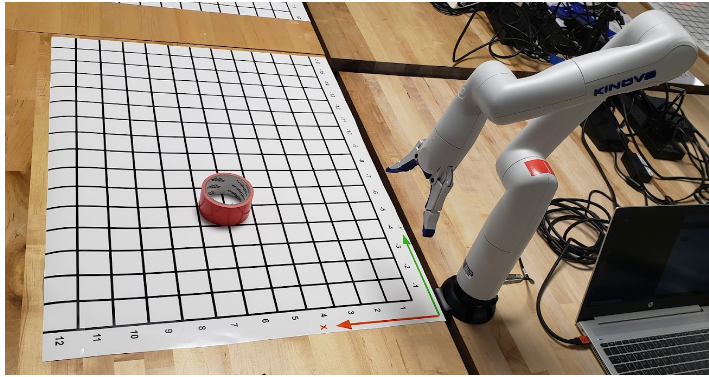
\includegraphics[width=10cm]{images/kinova.PNG}\vspace{-10pt}
    \caption{physical kinova arm.}\label{fig:gazebo}
    \end{figure}


\textbf{Instructions:}
\begin{enumerate}
    \item Open your browser and type your assigned robot’s IP address. This will open the Kinova Web App. The username is and the password are both "admin". 
    \begin{figure}[H]
    \vspace{-10pt}
    \centering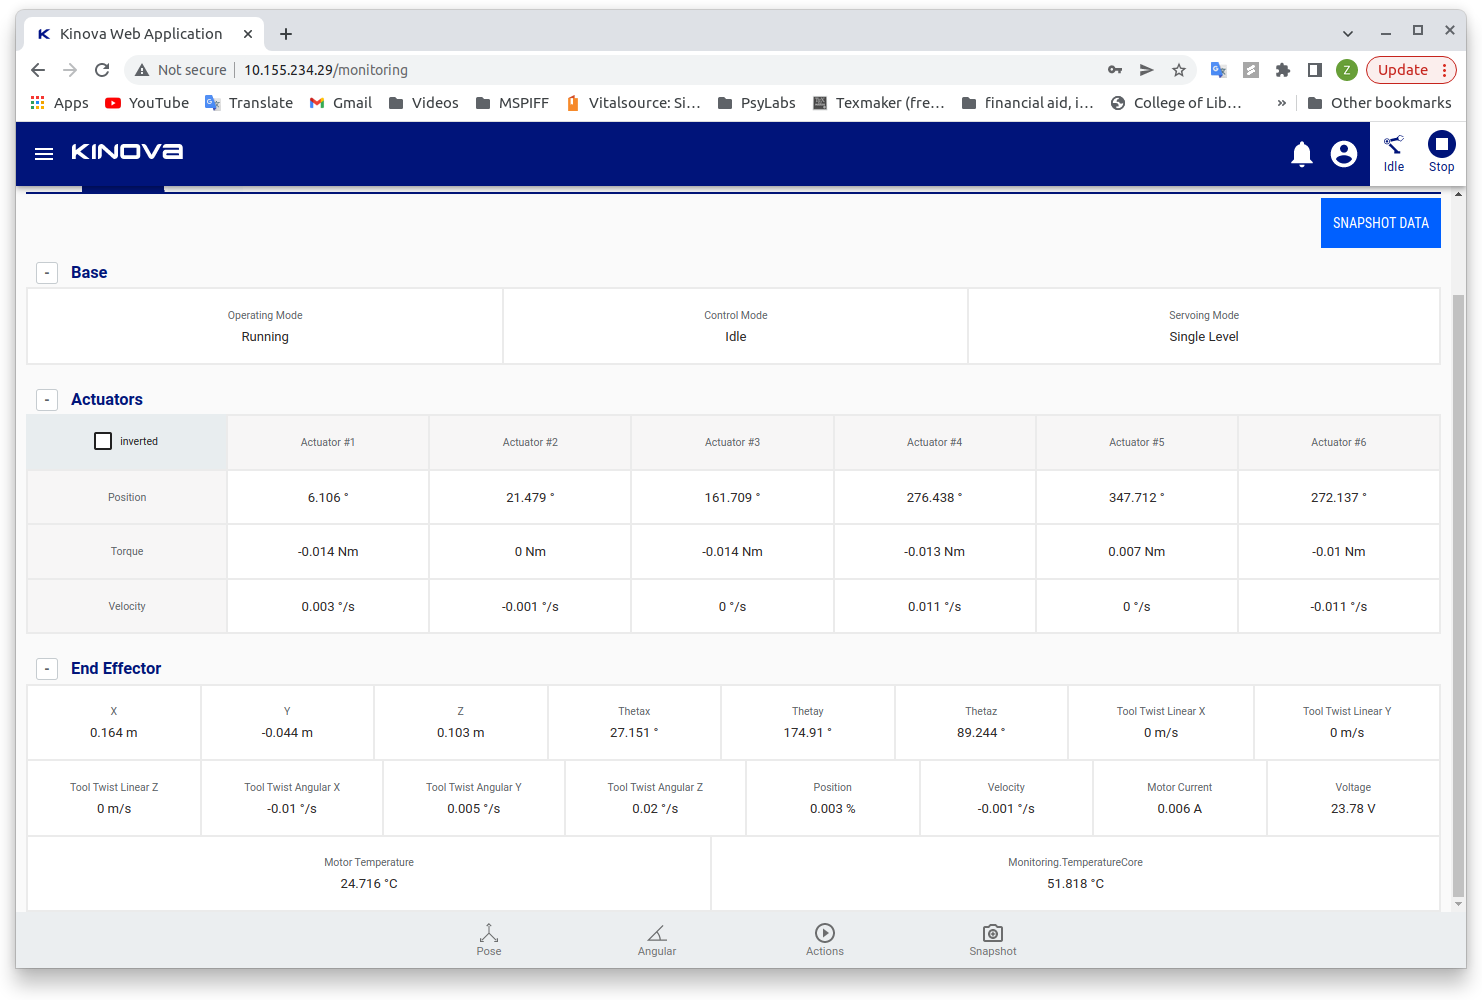
\includegraphics[width=12cm]{images/kinova1.PNG}\vspace{-10pt}
    \caption{kinova web app.}\label{fig:kinova1}
    \end{figure}
    
    \item In the Systems -> Monitoring you will see the current status of the robot’s joints: joint angle values, pose of the end effector with respect to the base, velocities and efforts for each joint.
    \item In the bottom panel there are two buttons: Pose and Angular. Each one of these, changes the position of the robot arm in a different working space: "Pose" changes the position and orientation of the end effector (task space), while "Angular" changes each joint angle value (configuration space).
    \begin{figure}[H]
    \vspace{-10pt}
    \centering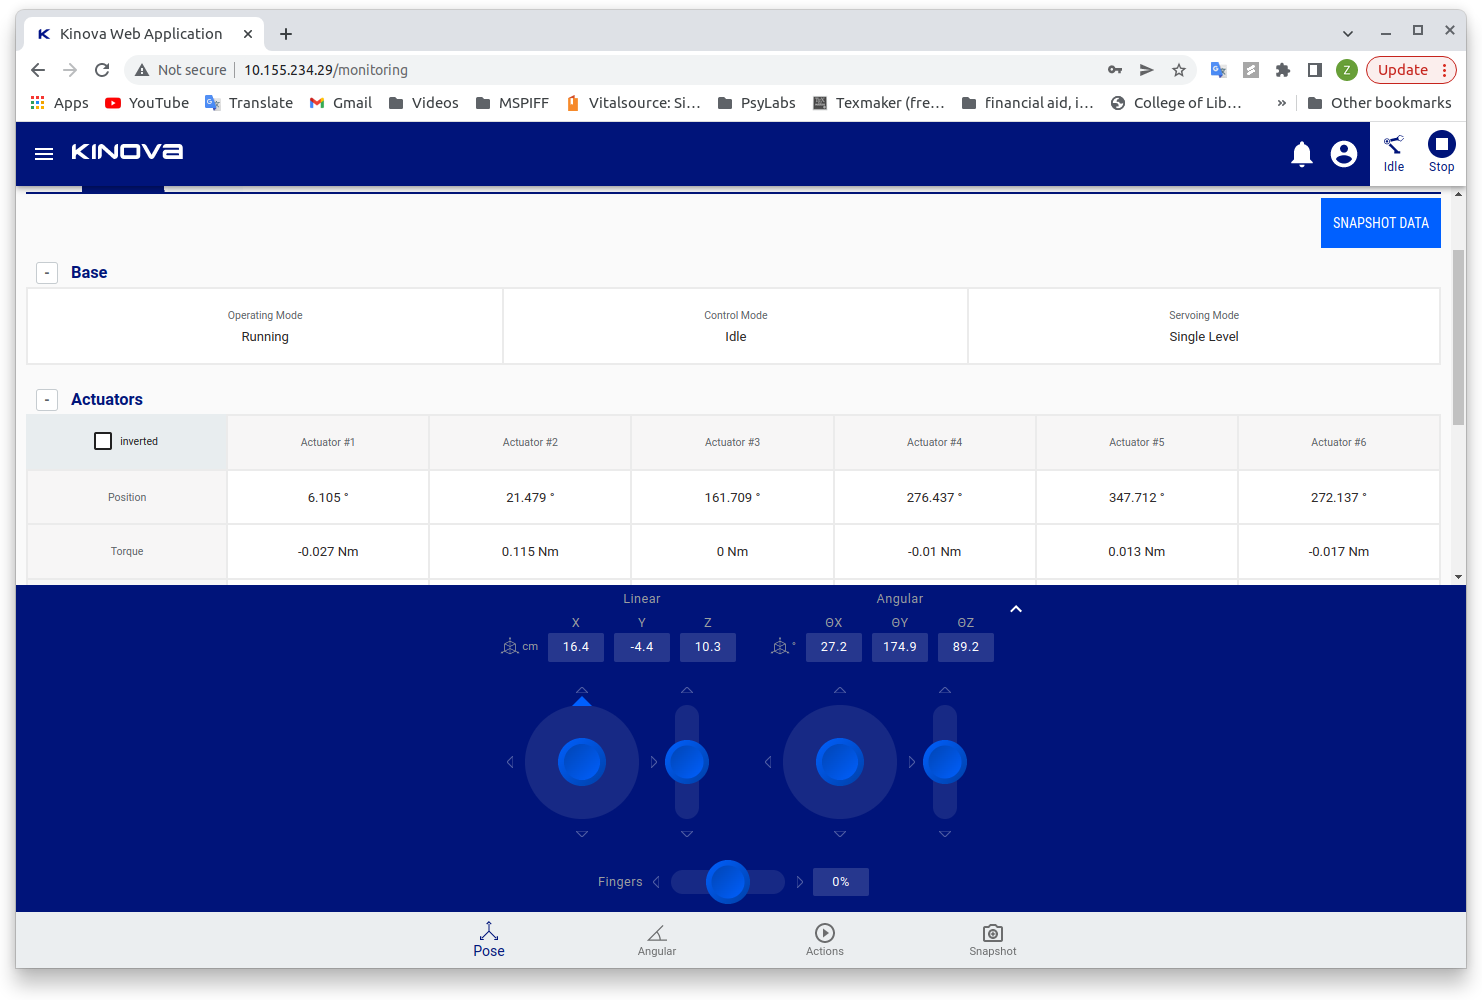
\includegraphics[width=12cm]{images/kinova2.PNG}\vspace{-10pt}
    \caption{kinova web app - work space.}\label{fig:kinova2}
    \end{figure}
    
    \begin{figure}[H]
    \vspace{-10pt}
    \centering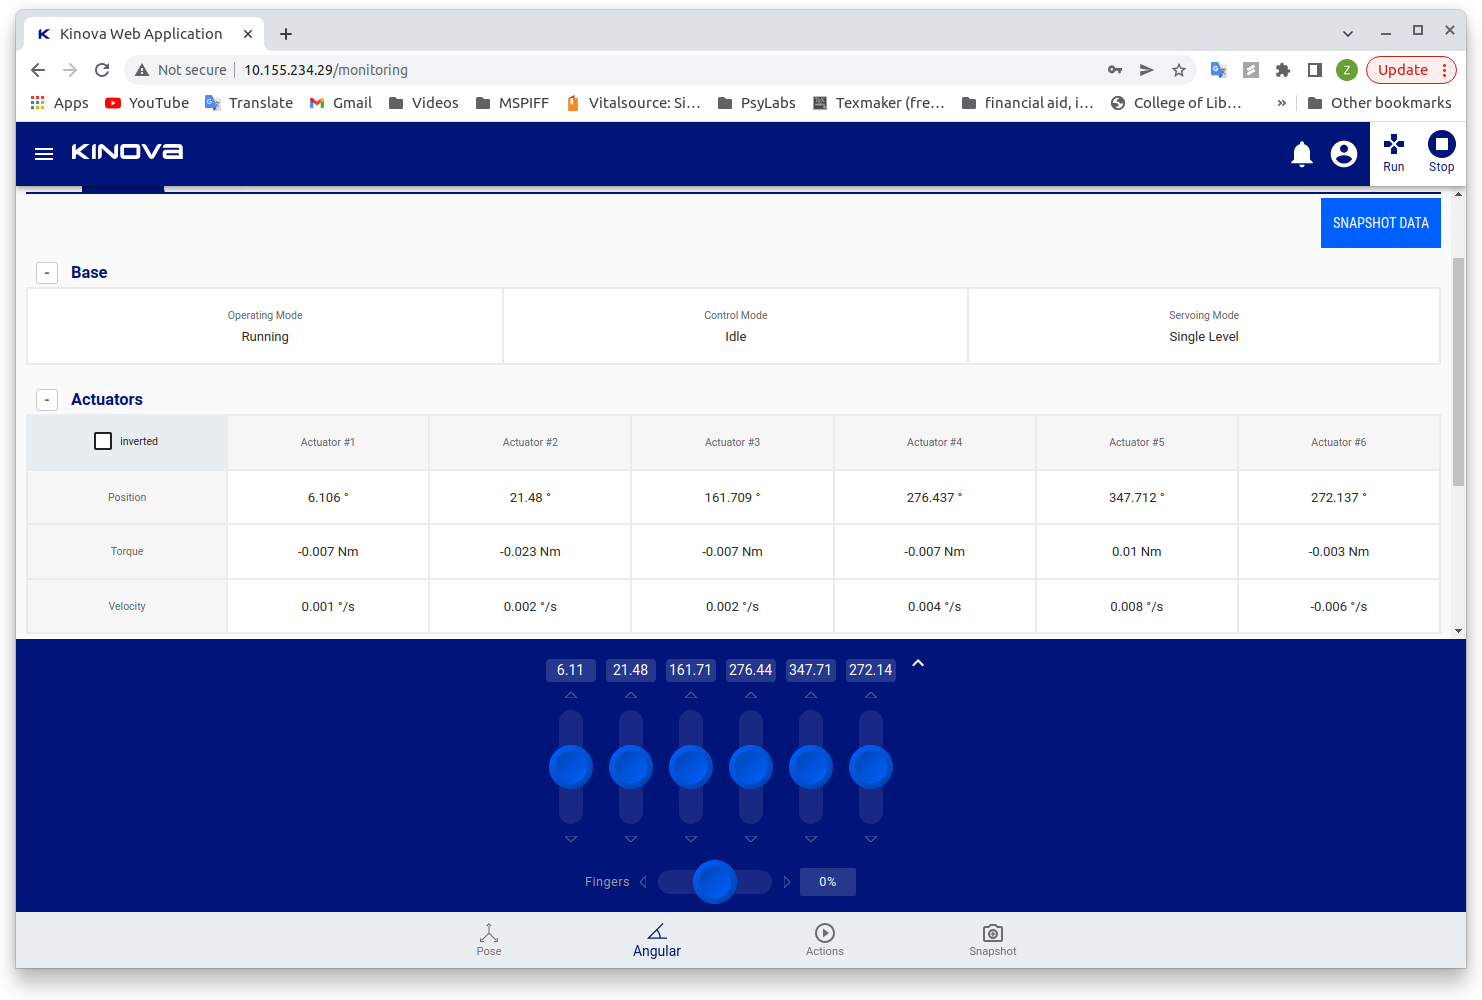
\includegraphics[width=12cm]{images/kinova3.PNG}\vspace{-10pt}
    \caption{kinova web app - configuration space (joint space).}\label{fig:kinova3}
    \end{figure}
\end{enumerate}
\textbf{Note}: Please be mindful as you use the UI’s joysticks and keep speeds low and movements small, particularly when movements lead towards the table. Please pay close attention to the robot motion and stop the motion using emergency stop if necessary. \\

\textbf{Deliverables:}
\begin{enumerate}
    \item Use the Pose tab on the bottom panel to move the robot’s end effector towards the Grid quadrant x = 4, y = 6. Select a z pose value greater than 15cm. Close the gripper to 10\%. You will have two camera views (one “over-the-shoulder” one “top”). Answering the following three questions:
    \begin{enumerate}
    \item Report the pose of the end effector (Position and Orientation with respect to the base).
    
    \begin{table}[H]
        \caption{Pose information of end effector at grid $(4, 6)$}
        \begin{subtable}{.5\linewidth}
            \centering
            \caption{Position}
            \begin{tabular}{cccc}
                \toprule
                \textbf{Linear} & \textit{x} & \textit{y} & \textit{z} \\\midrule
                \textbf{Position} & 20.2 & -30.3 & 54.9 \\\bottomrule
            \end{tabular}
        \end{subtable}
        \begin{subtable}{.5\linewidth}
            \centering
            \caption{Orientation}
            \begin{tabular}{cccc}
                \toprule
                \textbf{Angular} & \textit{$\theta$x} & \textit{$\theta$y} & \textit{$\theta$z} \\\midrule
                \textbf{Orientation} & 85.5 & 1.0 & 15.9 \\\bottomrule
            \end{tabular}
        \end{subtable}
    \end{table}

    \item What is the corresponding set of joint angles that match this pose?
    
    \begin{table}[H]
        \centering
        \caption{Joint angles of end effector at grid $(4, 6)$}
        \begin{tabular}{ccccccc}
        \toprule
        \textbf{Joint} & \textit{1} & \textit{2} & \textit{3} & \textit{4} & \textit{5} & \textit{6} \\ \midrule
        \textbf{Angle} & 317        & 284        & 248        & 55         & 116        & 249        \\ \bottomrule
        \end{tabular}
    \end{table}

    \item The grid on the table is 5cm x 5cm per square. Determine the transformation between the end-effector’s reference frame and the grid.
    
    \textbf{Answer: }The origin of the arm w.r.t. the grid quadrant is $(0, 12)$. Based on the information that the grid location $(4, 6)$ translates to pose $(20, -30)$, and that the grid is $5\times 5$, the formulae for transformation can be generalized as:
    \begin{multicols}{2}
        \noindent
        \begin{equation}
            x_{\text{pose}} = 5\times x_{\text{grid}}
        \end{equation}
        \begin{equation}
            y_{\text{pose}} = 5\times y_{\text{grid}} - 60
        \end{equation}
    \end{multicols}

    \end{enumerate}
    
    \item Take a photo of your robot reaching the required pose.
    
    \begin{figure}[h]
        \centering
        \subfloat[Front view]{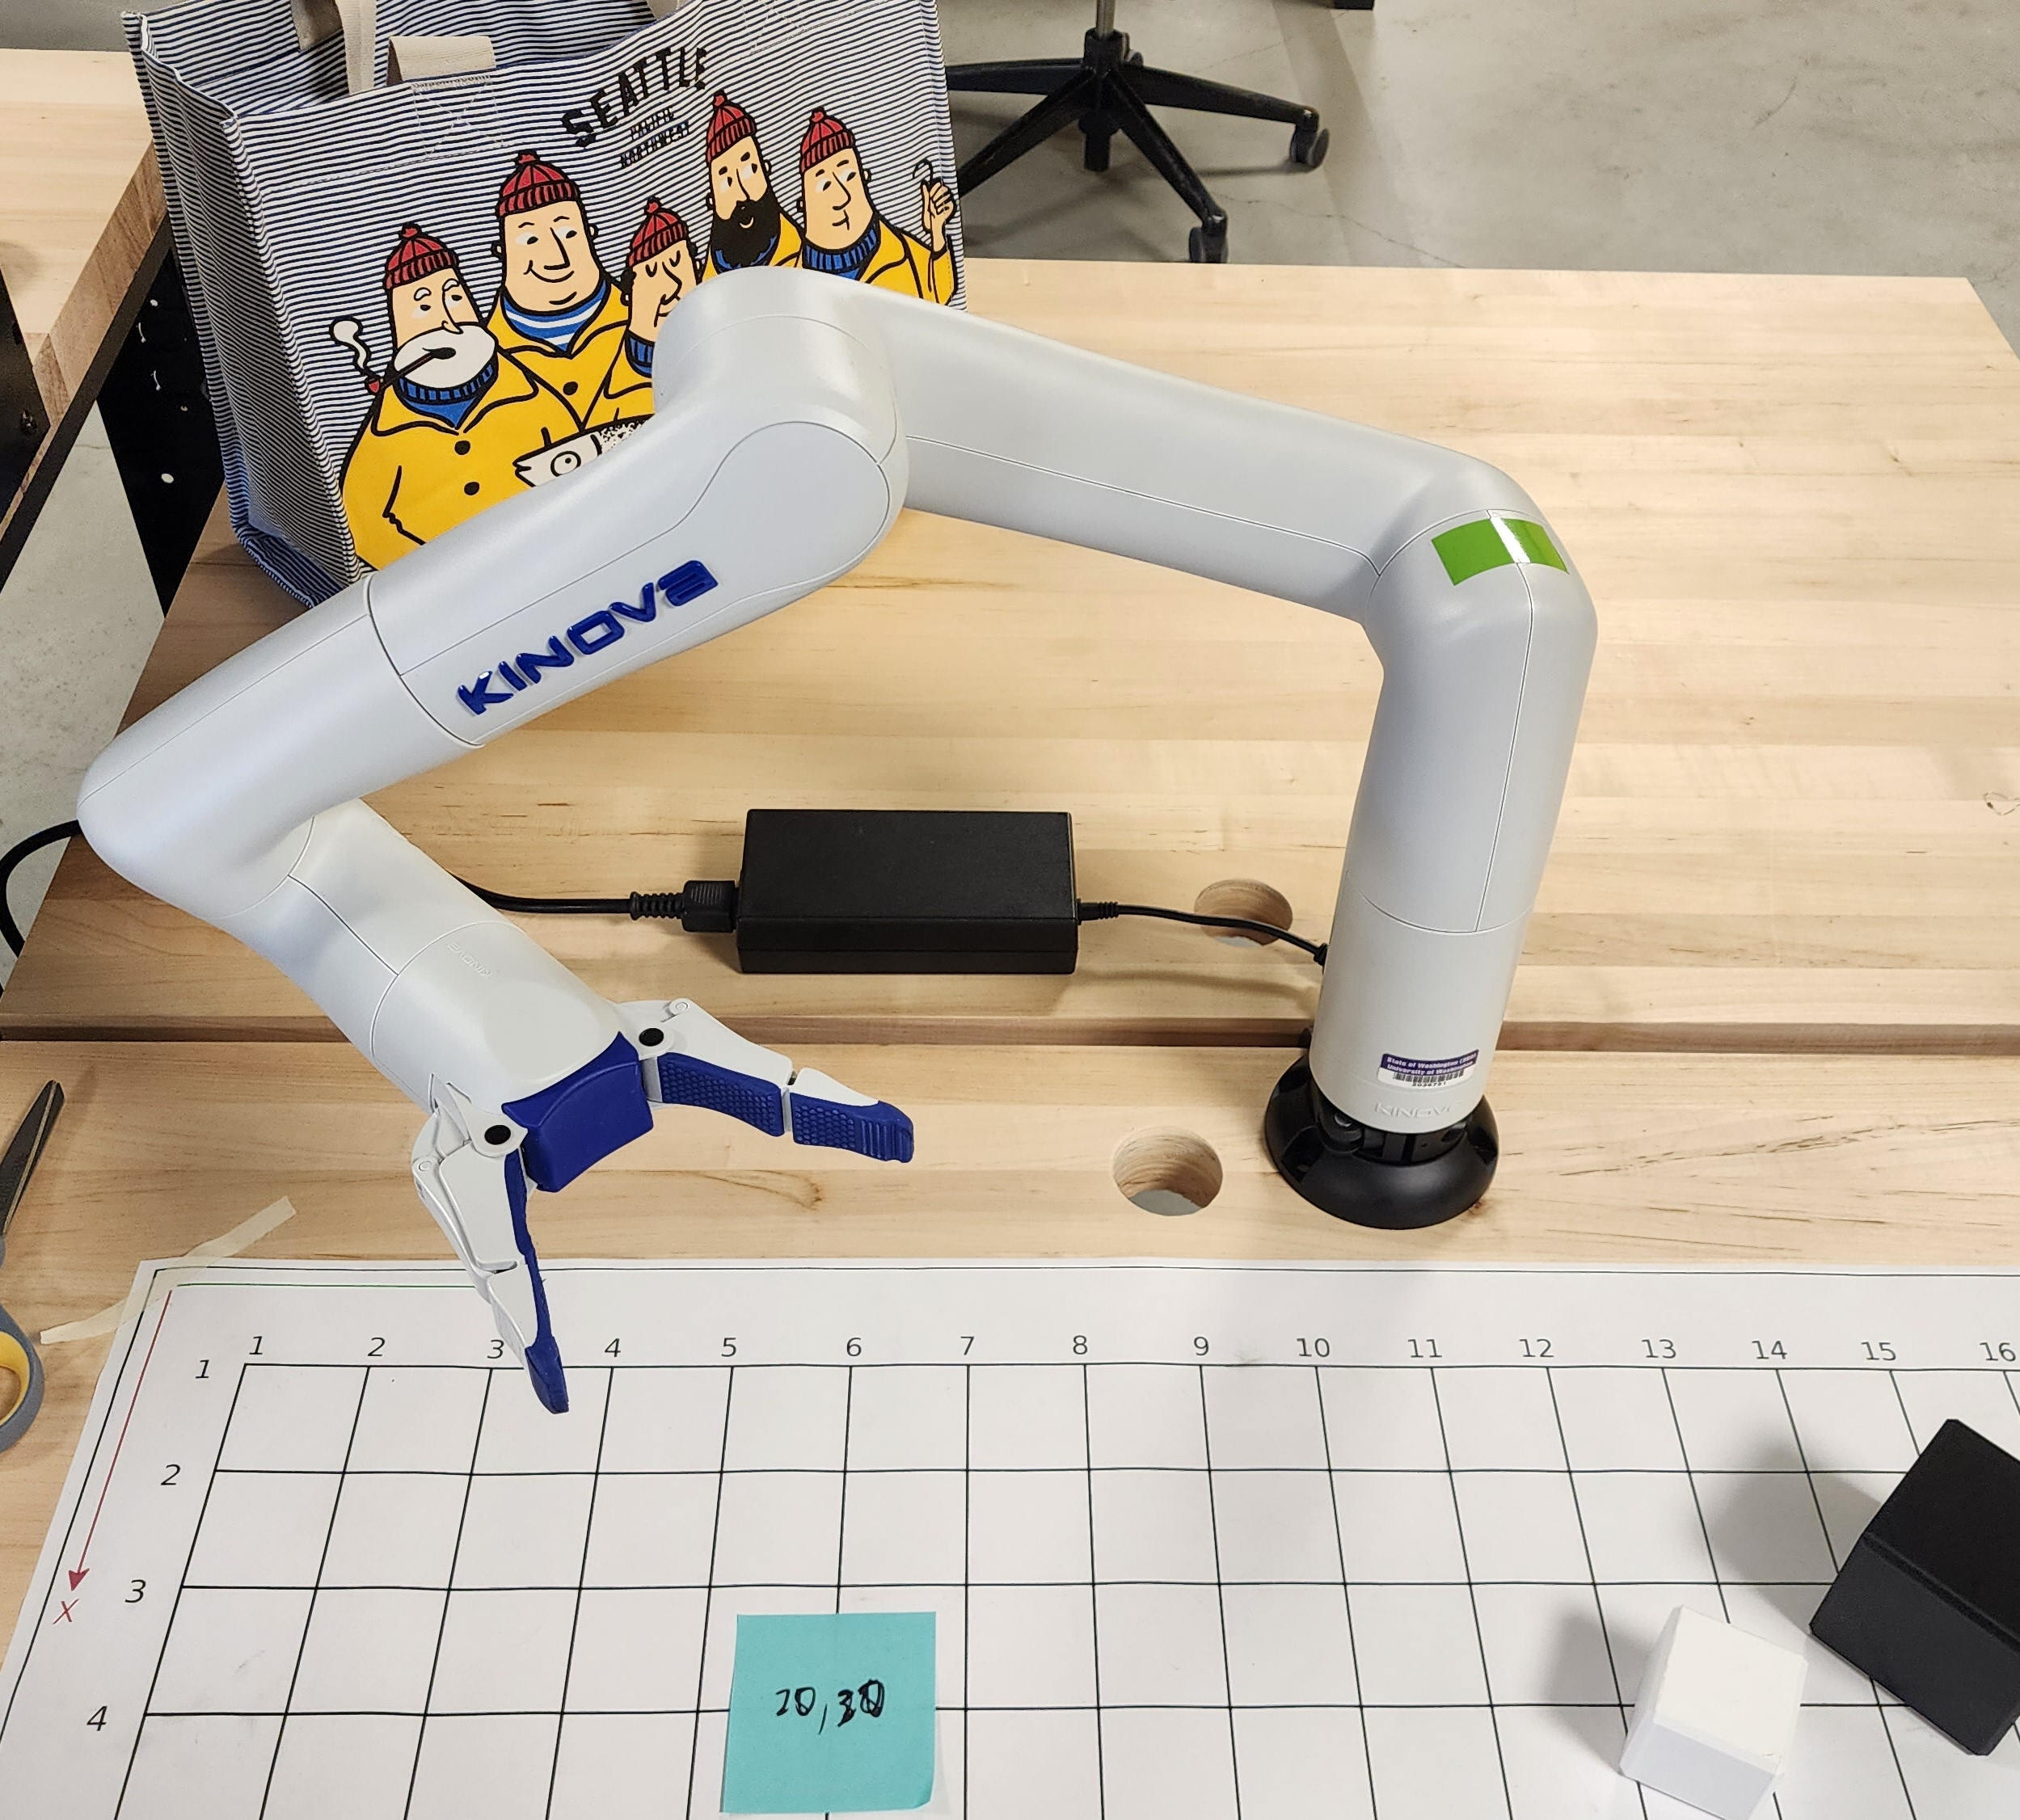
\includegraphics[height=5cm]{images/custom.jpeg}}
        \hspace{20pt}
        \subfloat[Bird view]{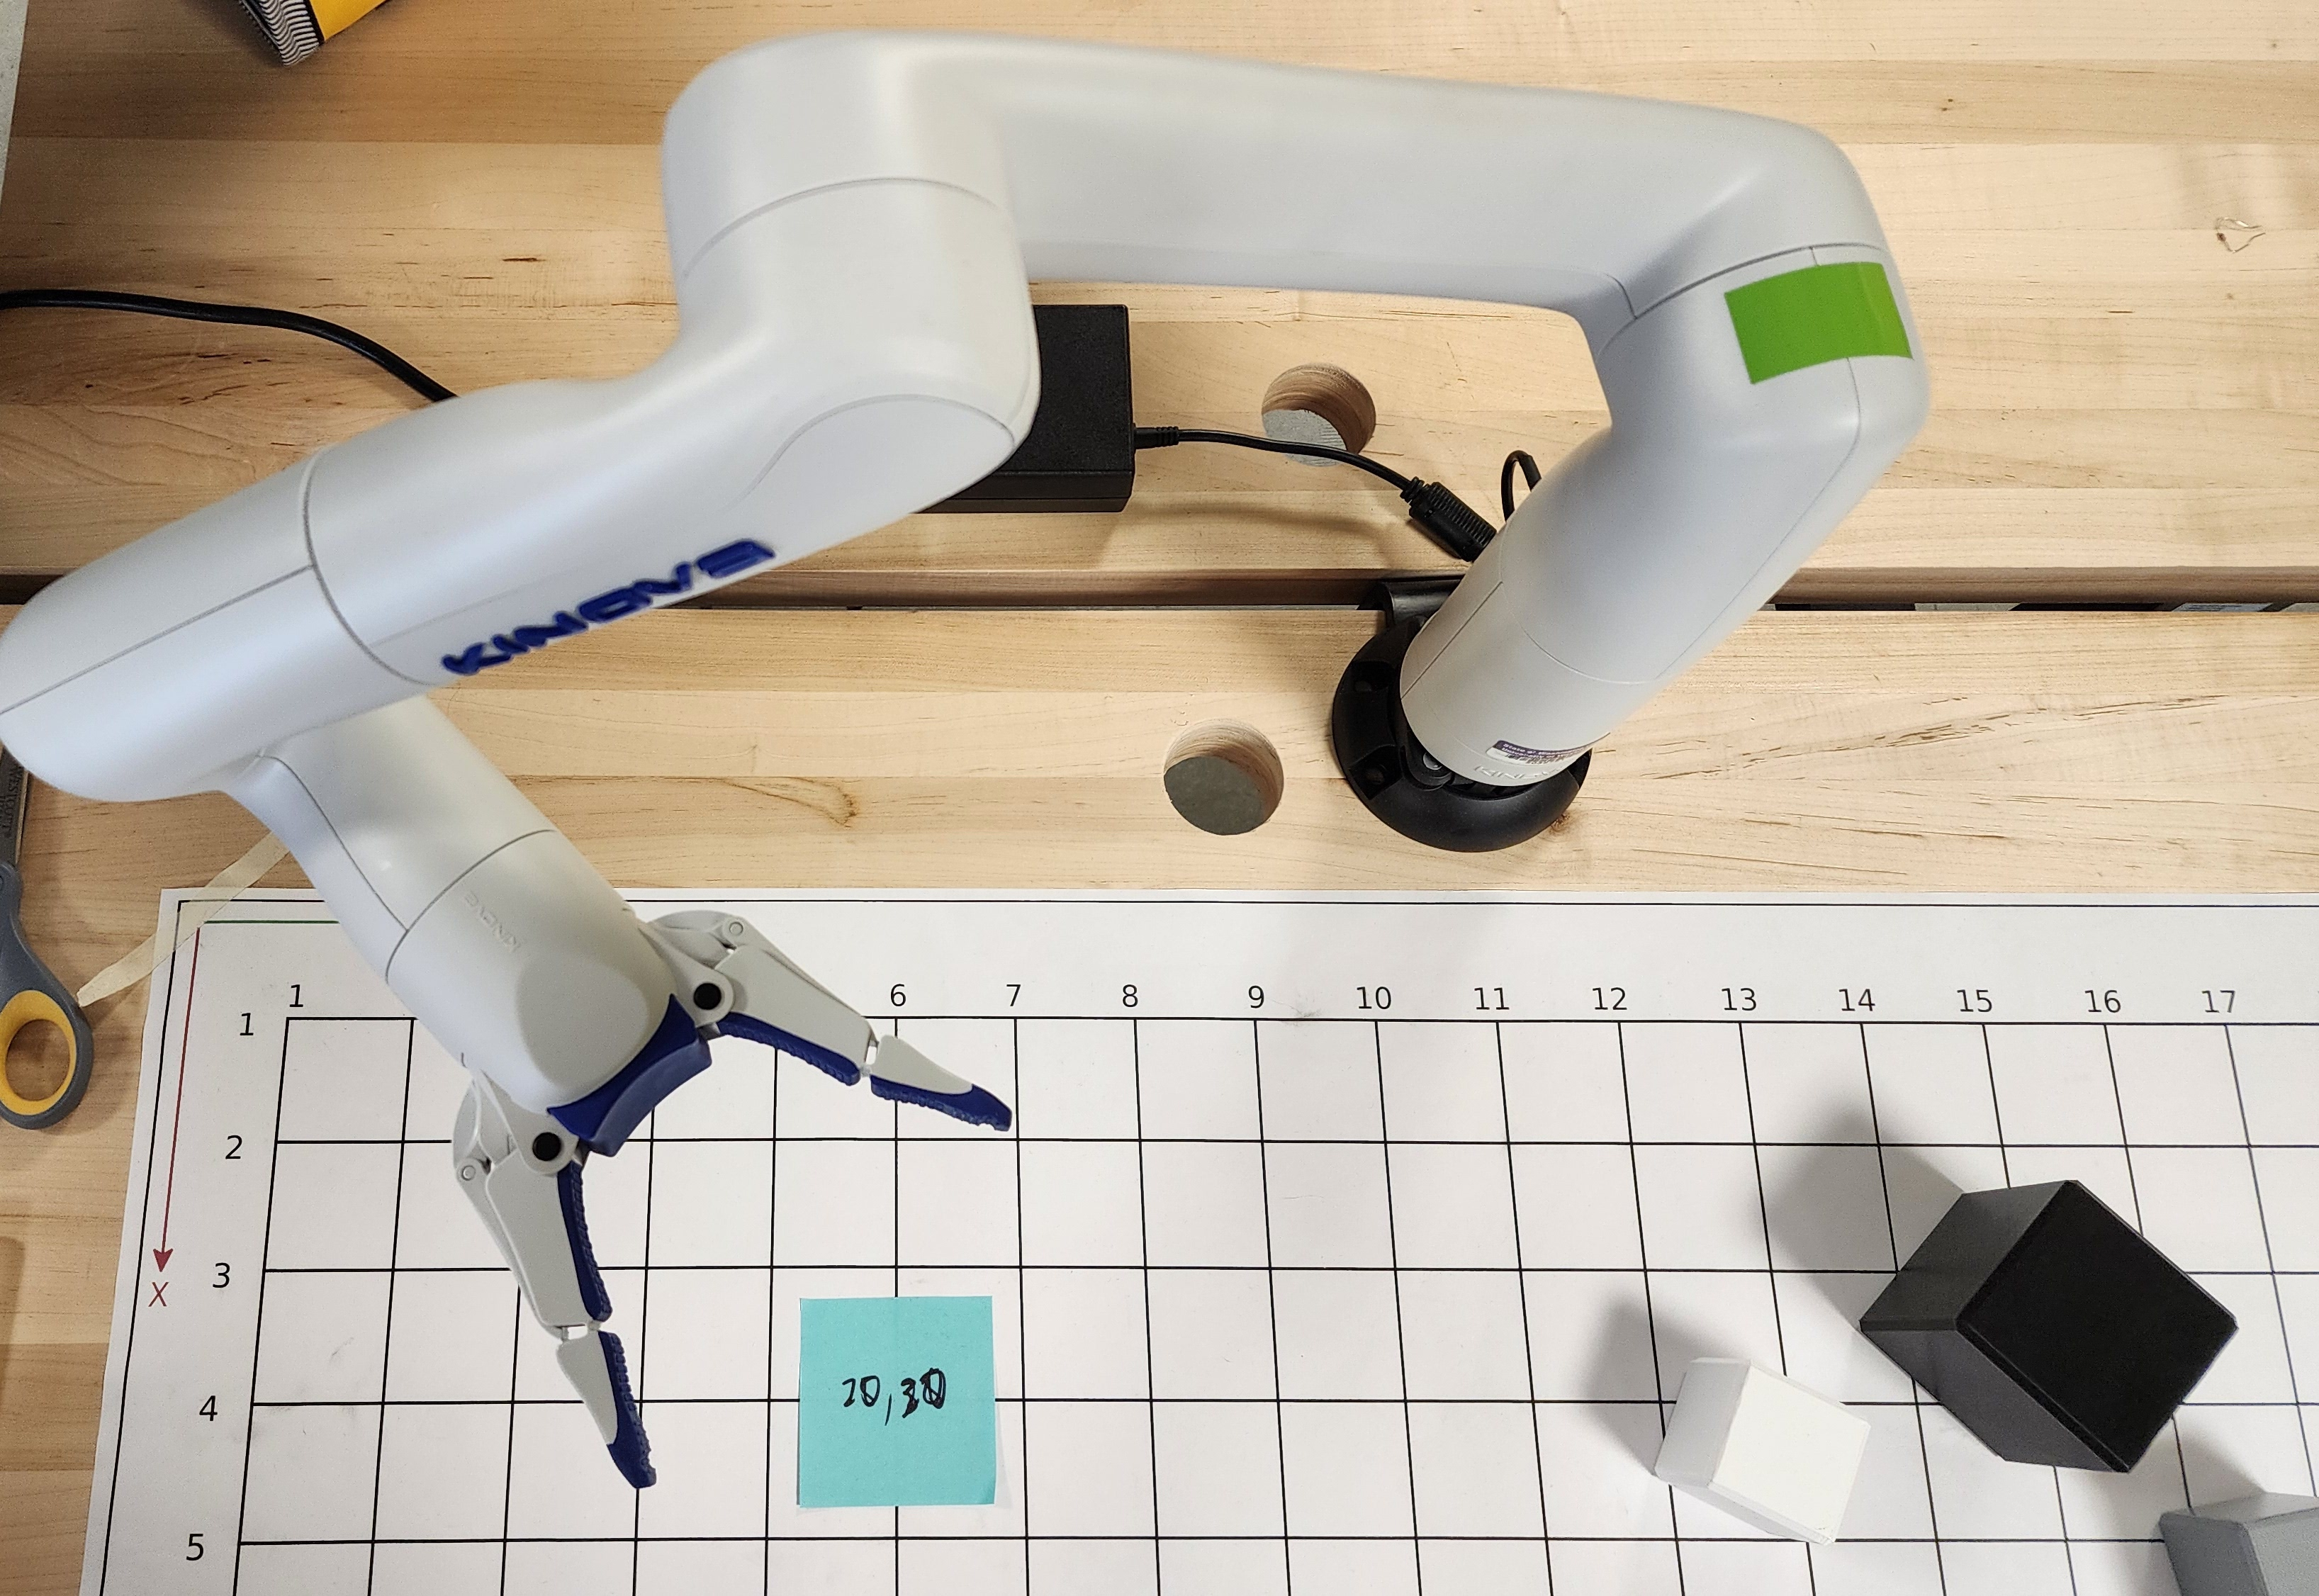
\includegraphics[height=5cm]{images/custom_1.jpeg}}
        \caption{Setting arm to reach custom goal state.}
        \label{fig:custom_arm}\vspace{-10pt}
    \end{figure}
    
    \item Switch to "Angular" on the bottom panel to move the robot to the following joint angle sets of values and report the robot’s pose of the end effector from either the Pose tab or from the Monitoring overview by taking a screenshot. Also provide your best estimate of the location from the Grid quadrant.
    
    \begin{enumerate}

    \item (17, 340, 134, 270, 338, 290) Gripper at 90\%
    
    \begin{table}[H]
        \caption{Pose information of end effector in custom state with grid estimate}
        \begin{subtable}{.3\linewidth}
            \centering
            \begin{tabular}{cccc}
                \toprule
                \textbf{Linear} & \textit{x} & \textit{y} & \textit{z} \\\midrule
                \textbf{Position} & 0.2 & 0.0 & 0.0 \\\bottomrule
            \end{tabular}
        \end{subtable}
        \hfill
        \begin{subtable}{.4\linewidth}
            \centering
            \begin{tabular}{cccc}
                \toprule
                \textbf{Angular} & \textit{$\theta$x} & \textit{$\theta$y} & \textit{$\theta$z} \\\midrule
                \textbf{Orientation} & 3.3 & 178.9 & 87.3 \\\bottomrule
            \end{tabular}
        \end{subtable}
        \hfill
        \begin{subtable}{.25\linewidth}
            \centering
            \begin{tabular}{cccc}
                \toprule
                \textbf{Linear} & \textit{x} & \textit{y} \\\midrule
                \textbf{Grid} & 0.04 & 12.00 \\\bottomrule
            \end{tabular}
        \end{subtable}
    \end{table}
    
    \item (357, 21, 150, 272, 320, 273) Gripper at 30\%
    
    \begin{table}[H]
        \caption{Pose information of end effector in retract state with grid estimate}
        \begin{subtable}{.3\linewidth}
            \centering
            \begin{tabular}{cccc}
                \toprule
                \textbf{Linear} & \textit{x} & \textit{y} & \textit{z} \\\midrule
                \textbf{Position} & 0.1 & -0.1 & 0.1 \\\bottomrule
            \end{tabular}
        \end{subtable}
        \hfill
        \begin{subtable}{.4\linewidth}
            \centering
            \begin{tabular}{cccc}
                \toprule
                \textbf{Angular} & \textit{$\theta$x} & \textit{$\theta$y} & \textit{$\theta$z} \\\midrule
                \textbf{Orientation} & 10.8 & 177.9 & 82.8 \\\bottomrule
            \end{tabular}
        \end{subtable}
        \hfill
        \begin{subtable}{.25\linewidth}
            \centering
            \begin{tabular}{cccc}
                \toprule
                \textbf{Linear} & \textit{x} & \textit{y} \\\midrule
                \textbf{Grid} & 0.02 & 12.02 \\\bottomrule
            \end{tabular}
        \end{subtable}
    \end{table}

    \begin{figure}[]
        \centering
        \subfloat[Custom state]{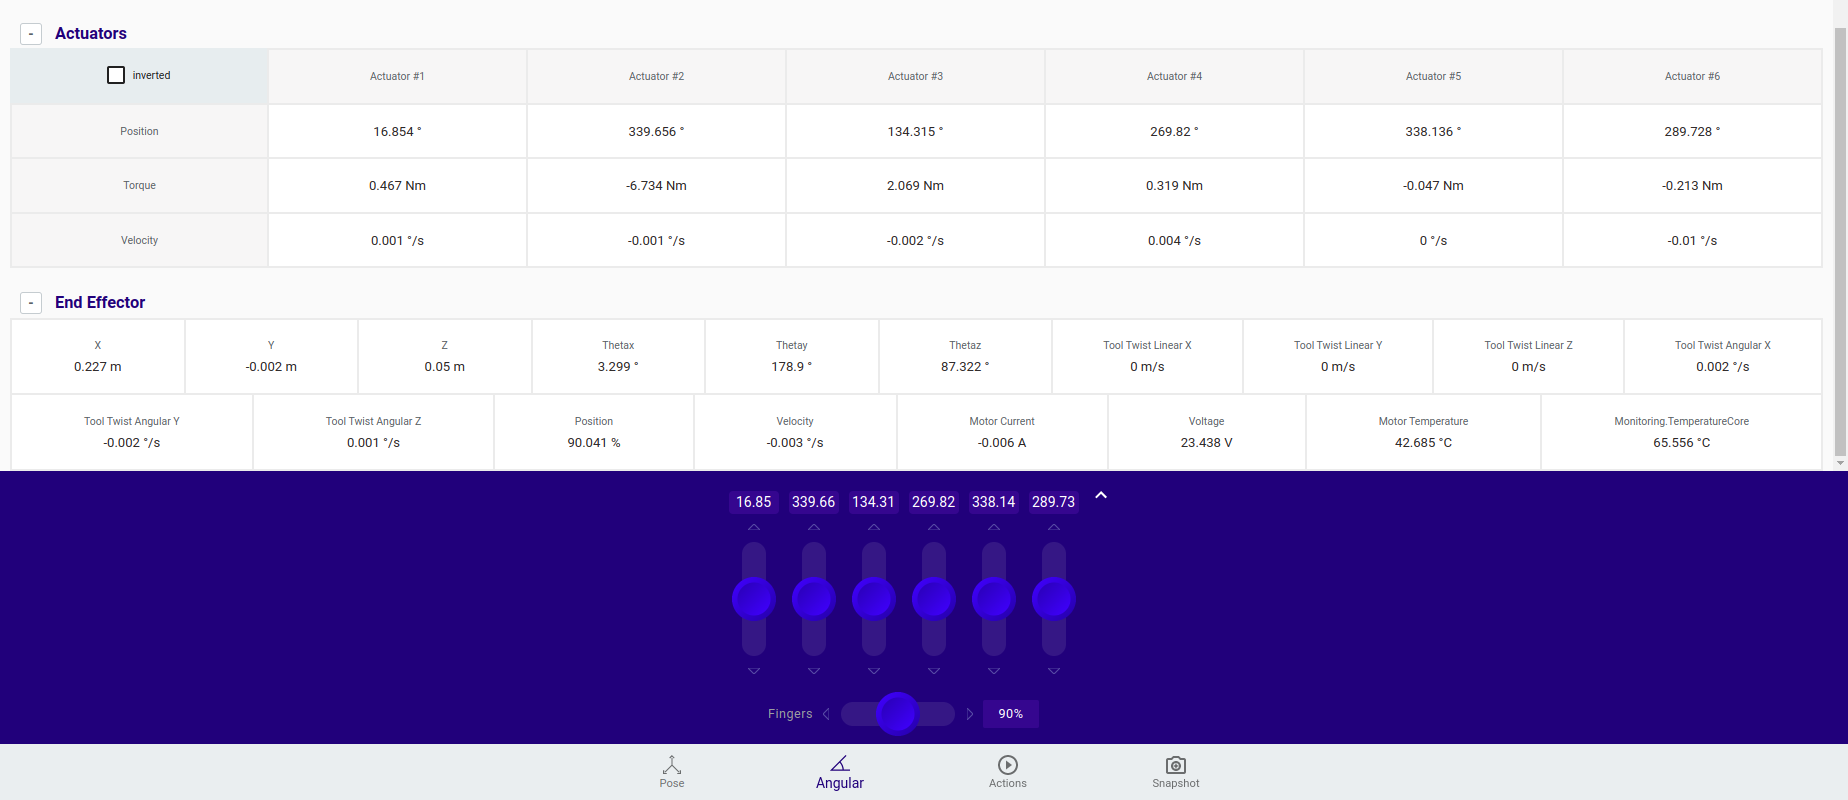
\includegraphics[width=0.48\linewidth]{images/custom_web.png}}
        \hfill
        \subfloat[Retract state]{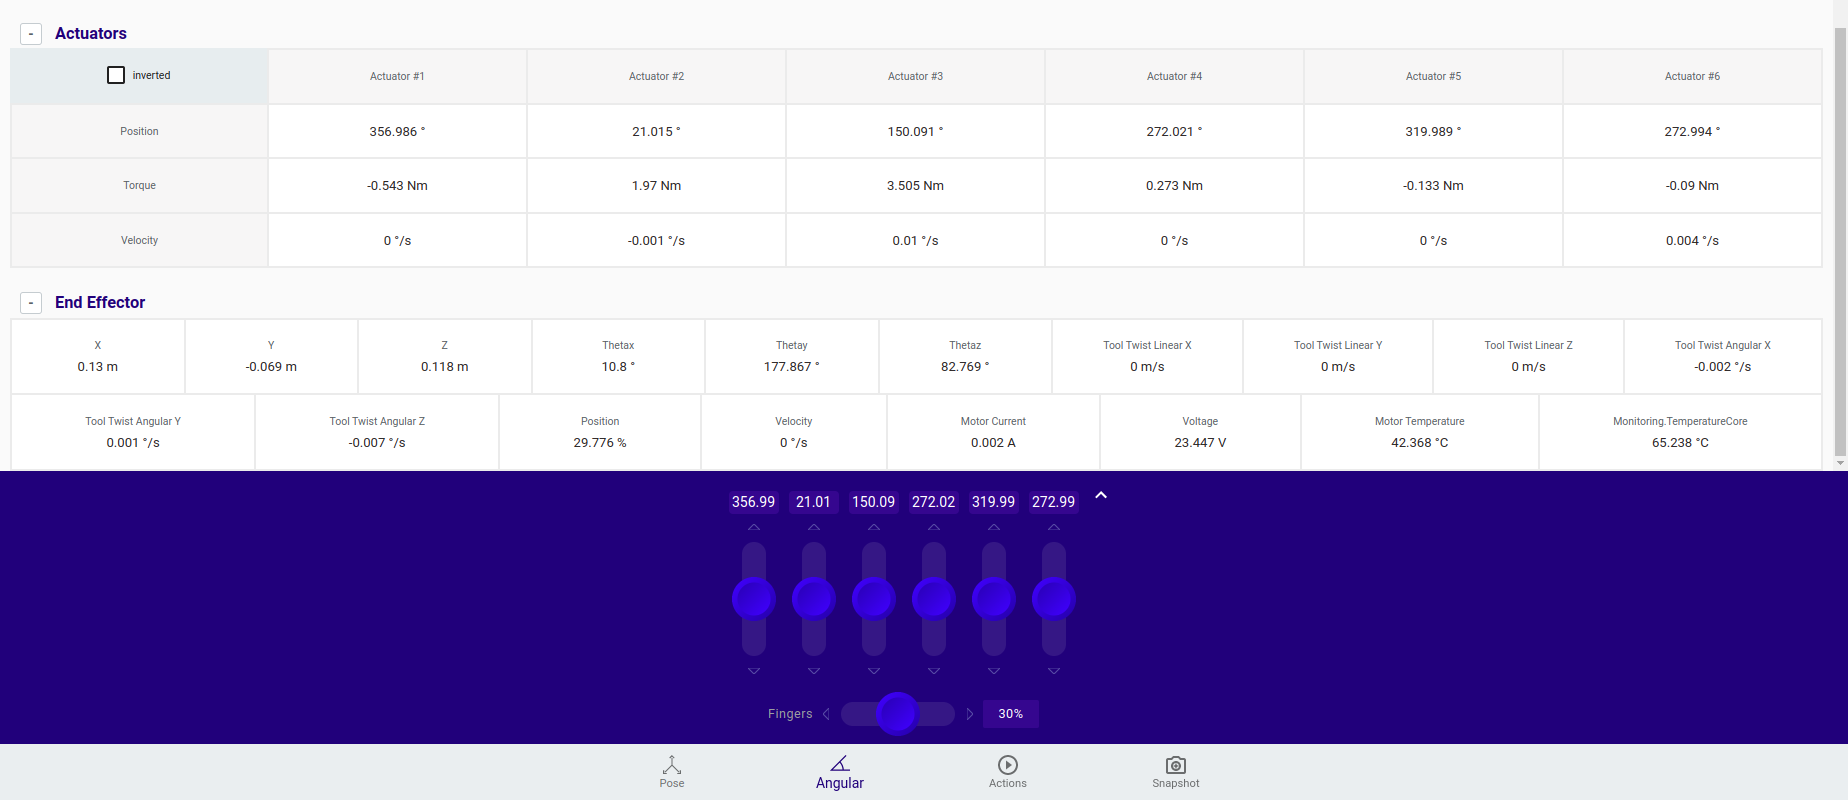
\includegraphics[width=0.48\linewidth]{images/retract_web.png}}
        \caption{Monitoring Pose of the end effector.}
        \label{fig:custom_arm}\vspace{-10pt}
    \end{figure}

    \end{enumerate}
\end{enumerate}


\subsection{Spawning a Kinova robot arm using Kortex Driver}

We will use the ros\_kortex repository to work with the Kinova arm. In this metapackage, we will use the kortex\_driver portion. Execute the following launch file that will bring up the gen3\_lite controllers, MoveIt! Configurations and an RViZ window.

\begin{minted}{bash}
        ~$ roslaunch kortex_driver kortex_driver.launch arm:=gen3_lite ip_address:=
        <IP OF ROBOT>
    \end{minted}

\textbf{Note:} Once the RViZ window has been opened, and the terminal should show two green messages ( “You can start planning now!” and “The Kortex driver has been initialized correctly!” ). At this point, you can add a MotionPlanning component in RviZ.

\begin{figure}[H]
    \centering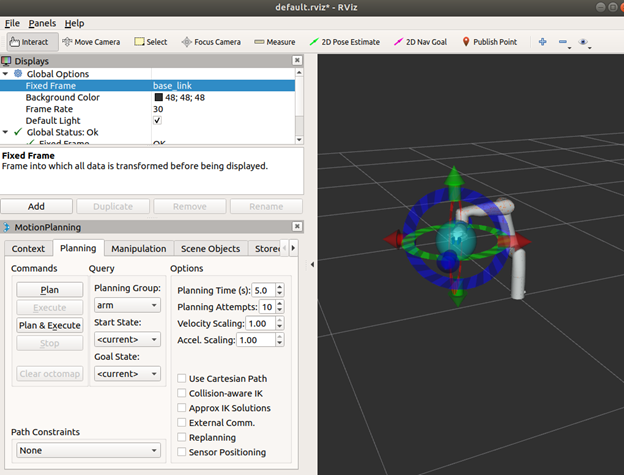
\includegraphics[width=10cm]{images/kinovaRviz.png}
    \caption{Kinova Rviz.}\label{fig:kinovarviz}\vspace{-10pt}
    \end{figure}


\subsection{Using the Interactive Markers to change the robot’s pose based on the cartesian-space}

\textbf{Instructions:}

\begin{enumerate}

    \item You can use the different arrows and rings in the RViZ interactive marker, to change position and orientation of the robot’s end-effector. As you use them, you will see an orange version of the robot arm with the proposed new position. Once you have reached a desired position, use the buttons “Plan” and “Execute” to make the robot in Gazebo match the new proposed position. Some useful tools for you to track the robot’s motions are:
    
    \begin{minted}{bash}
        ~$ rostopic echo -n 1 /my_gen3_lite/joint_states
    \end{minted}

    which publishes the values of the joints.
    
    \begin{minted}{bash}
        ~$ rosrun tf tf_echo /base_link <END-EFFECTOR LINK>
    \end{minted}
    
    which outputs the pose of the robot’s end-effector with respect to the base of the robot. You may also come to realize that there are other links on the robot’s gripper that might report different values. You can use the following command to generate a PDF with the TF tree for the robot:
    
    \begin{minted}{bash}
        ~$ rosrun tf view_frames
    \end{minted}
    
    \item If you want to change the state of the gripper, you need to change the Planning Group from arm to gripper, and you can select a new position.

\end{enumerate}

\textbf{Deliverables:}

\begin{enumerate}

    \item What are the reported robot’s joints values and end-effector pose (position and orientation w.r.t. the base, consider using both end\_effector\_link and tool\_frame links) when you send the arm to the following positions:
    
    \begin{enumerate}

        \item Home
        
        \begin{table}[H]
            \caption{Pose information of end effector in home state}
            \begin{subtable}{.4\linewidth}
                \centering
                \caption{Position}
                \begin{tabular}{cccc}
                    \toprule
                    Source & \textit{x} & \textit{y} & \textit{z} \\\midrule
                    end\_effector\_link & 0.37 & 0.08 & 0.45 \\
                    tool\_frame\_link & 0.44 & 0.19 & 0.45 \\
                    Kinova Web App & 0.44 & 0.19 & 0.45 \\\bottomrule
                \end{tabular}
            \end{subtable}
            \hfill
            \begin{subtable}{.52\linewidth}
                \centering
                \caption{Orientation}
                \begin{tabular}{ccccc}
                    \toprule
                    Source & \textit{x} & \textit{y} & \textit{z} & \textit{w} \\\midrule
                    end\_effector\_link & -0.35 & 0.62 & 0.36 & 0.61 \\
                    tool\_frame\_link & 0.19 & 0.69 & 0.68 & 0.18 \\\bottomrule
                \end{tabular}
            \end{subtable}
        \end{table}
        \vspace{-10pt}
        \begin{table}[H]
            \centering
            \caption{Joint angles of end effector in home state}
            \begin{tabular}{ccccccc}
            \toprule
            Source & \textit{1} & \textit{2} & \textit{3} & \textit{4} & \textit{5} & \textit{6} \\\midrule
            joint\_states & 0.00 & -0.28 & 1.31 & 0.00 & -1.05 & 0.00 \\
            RViz & 0 & -16 & 75 & 0 & -60 & 0 \\
            Kinova Web App & 360 & 344 & 75 & 360 & 300 & 0 \\\bottomrule
            \end{tabular}
        \end{table}

        \item Vertical
        
        \begin{table}[H]
            \caption{Pose information of end effector in vertical state}
            \begin{subtable}{.4\linewidth}
                \centering
                \caption{Position}
                \begin{tabular}{cccc}
                    \toprule
                    Source & \textit{x} & \textit{y} & \textit{z} \\\midrule
                    end\_effector\_link & 0.06 & -0.01 & 0.87 \\
                    tool\_frame\_link & 0.06 & -0.01 & 1.00 \\
                    Kinova Web App & 0.06 & -0.01 & 1.00 \\\bottomrule
                \end{tabular}
            \end{subtable}
            \hfill
            \begin{subtable}{.52\linewidth}
                \centering
                \caption{Orientation}
                \begin{tabular}{ccccc}
                    \toprule
                    Source & \textit{x} & \textit{y} & \textit{z} & \textit{w} \\\midrule
                    end\_effector\_link & 0.00 & 0.00 & 0.00 & 1 \\
                    tool\_frame\_link & 0.00 & 0.00 & 0.71 & 0.71 \\\bottomrule
                \end{tabular}
            \end{subtable}
        \end{table}
        \vspace{-10pt}
        \begin{table}[H]
            \centering
            \caption{Joint angles of end effector in vertical state}
            \begin{tabular}{ccccccc}
            \toprule
            Source & \textit{1} & \textit{2} & \textit{3} & \textit{4} & \textit{5} & \textit{6} \\\midrule
            joint\_states & 0.00 & 0.00 & 0.00 & 0.00 & 0.00 & 0.00 \\
            RViz & 0 & 0 & 0 & 0 & 0 & 0 \\
            Kinova Web App & 360 & 360 & 360 & 360 & 0 & 0 \\\bottomrule
            \end{tabular}
        \end{table}

        \item Grid quadrant x = 4, y = 6. Note: Keep the z-pose value greater than 15cm to avoid hitting the ground.

        \begin{table}[H]
            \caption{Pose information of end effector at grid $(4, 6)$}
            \begin{subtable}{.4\linewidth}
                \centering
                \caption{Position}
                \begin{tabular}{cccc}
                    \toprule
                    Source & \textit{x} & \textit{y} & \textit{z} \\\midrule
                    end\_effector\_link & 0.17 & -0.18 & 0.54 \\
                    tool\_frame\_link & 0.20 & -0.30 & 0.55 \\
                    Kinova Web App & 0.20 & -0.30 & 0.55 \\\bottomrule
                \end{tabular}
            \end{subtable}
            \hfill
            \begin{subtable}{.52\linewidth}
                \centering
                \caption{Orientation}
                \begin{tabular}{ccccc}
                    \toprule
                    Source & \textit{x} & \textit{y} & \textit{z} & \textit{w} \\\midrule
                    end\_effector\_link & 0.40 & 0.55 & 0.45 & 0.58 \\
                    tool\_frame\_link & 0.67 & 0.10 & 0.10 & 0.73 \\\bottomrule
                \end{tabular}
            \end{subtable}
        \end{table}
        \vspace{-10pt}
        \begin{table}[H]
            \centering
            \caption{Joint angles of end effector at grid $(4, 6)$}
            \begin{tabular}{ccccccc}
            \toprule
            Source & \textit{1} & \textit{2} & \textit{3} & \textit{4} & \textit{5} & \textit{6} \\\midrule
            joint\_states & -0.75 & -1.33 & -1.95 & 0.96 & 2.02 & -1.94 \\
            RViz & -43 & -76 & -112 & 55 & 116 & -111 \\
            Kinova Web App & 317 & 284 & 248 & 55 & 116 & 249 \\\bottomrule
            \end{tabular}
        \end{table}
    
    \item Compare the results reported by the Kinova Web App Monitoring against the reported values from tf\_echo and joint\_states for the 3 previous positions. Discuss any potential source for difference in the two sources. You can take screenshots to compare. 
    
    \textbf{Answer: }As can be seen in the tables above, there are differences and similarities between the values reported in Kinova and RViz/Terminal. The relationships between them can be found and summarized as:

        \begin{enumerate}

            \item For position values in Pose, the end\_effector is different from, while tool\_frame is the same as, the end effector position in Kinova GUI. Having different definitions of the end effector, RViz and Kinova report positions of distinct parts. 
            \\Specifically, end effector in Kinova refer to the \textit{tool} at the end of the robot, in this case a gripper, that directly interacts with the environment; however, end effector in RViz is the same as joint\_6 in joint\_states, the last joint of the robot.
            
            \item For joint values, all of them display different yet the same results. The angle range of Kinova is the original $[0, 360]$, whereas that of the RViz is $[-180, 180]$.
            \\Conversion from Kinova to RViz joint state isn't hard: when the angle is above $180^\circ$, subtract $360$ from it; when below, keep it as is. The joint positions returned by joint\_states, on the other hand, are just the radian values converted from the degree values in RViz.
        
        \end{enumerate}

    \end{enumerate}

\end{enumerate}


\subsection{Using the Joints tab in MotionPlanning to change the robot’s pose on the configuration-space}

\textbf{Instructions:}

In the Motion Planning component, find the Joints tab. You will be able to change the values of the different joint angles. Explore the configuration space, determine which joints move in which direction when a positive or a negative angle is given to each joint.\\

\textbf{Deliverables:}
\begin{enumerate}
    \item Use the same tools (tf\_echo, joint\_states, and the reported values in the Kinova Web App) described in the previous subsections to explore the values for the pose and the joint angles of the following sets:
    \begin{enumerate}
        \item (17, 340, 134, 270, 338, 290) Gripper at 90\%
        
        \begin{table}[H]
            \caption{Pose information of end effector in custom state}
            \begin{subtable}{.4\linewidth}
                \centering
                \caption{Position}
                \begin{tabular}{cccc}
                    \toprule
                    Source & \textit{x} & \textit{y} & \textit{z} \\\midrule
                    end\_effector\_link & 0.22 & 0.00 & 0.18 \\
                    tool\_frame\_link & 0.23 & 0.00 & 0.05 \\
                    Kinova Web App & 0.23 & 0.00 & 0.05 \\\bottomrule
                \end{tabular}
            \end{subtable}
            \hfill
            \begin{subtable}{.52\linewidth}
                \centering
                \caption{Orientation}
                \begin{tabular}{ccccc}
                    \toprule
                    Source & \textit{x} & \textit{y} & \textit{z} & \textit{w} \\\midrule
                    end\_effector\_link & 1.00 & -0.02 & 0.04 & -0.01 \\
                    tool\_frame\_link & -0.69 & 0.72 & -0.02 & 0.03 \\\bottomrule
                \end{tabular}
            \end{subtable}
        \end{table}
        \vspace{-10pt}
        \begin{table}[H]
            \centering
            \caption{Joint angles of end effector in custom state}
            \begin{tabular}{ccccccc}
            \toprule
            Source & \textit{1} & \textit{2} & \textit{3} & \textit{4} & \textit{5} & \textit{6} \\\midrule
            joint\_states & 0.30 & -0.35 & 2.34 & -1.57 & -0.38 & -1.22 \\
            RViz & 17 & -20 & 134 & -90 & -22 & -70 \\
            Kinova Web App & 17 & 340 & 134 & 270 & 338 & 290 \\\bottomrule
            \end{tabular}
        \end{table}

        \item (357, 21, 150, 272, 320, 273) Gripper at 30\%
        
        \begin{table}[H]
            \caption{Pose information of end effector in retract state}
            \begin{subtable}{.4\linewidth}
                \centering
                \caption{Position}
                \begin{tabular}{cccc}
                    \toprule
                    Source & \textit{x} & \textit{y} & \textit{z} \\\midrule
                    end\_effector\_link & 0.11 & -0.07 & 0.25 \\
                    tool\_frame\_link & 0.13 & -0.07 & 0.12 \\
                    Kinova Web App & 0.13 & -0.07 & 0.12 \\\bottomrule
                \end{tabular}
            \end{subtable}
            \hfill
            \begin{subtable}{.52\linewidth}
                \centering
                \caption{Orientation}
                \begin{tabular}{ccccc}
                    \toprule
                    Source & \textit{x} & \textit{y} & \textit{z} & \textit{w} \\\midrule
                    end\_effector\_link & 0.99 & -0.06 & 0.10 & -0.01 \\
                    tool\_frame\_link & -0.66 & 0.75 & -0.06 & 0.08 \\\bottomrule
                \end{tabular}
            \end{subtable}
        \end{table}
        \vspace{-10pt}
        \begin{table}[H]
            \centering
            \caption{Joint angles of end effector in vertical state}
            \begin{tabular}{ccccccc}
            \toprule
            Source & \textit{1} & \textit{2} & \textit{3} & \textit{4} & \textit{5} & \textit{6} \\\midrule
            joint\_states & -0.05 & 0.37 & 2.62 & -1.54 & -0.70 & -1.52 \\
            RViz & -3 & 21 & 150 & -88 & -40 & -87 \\
            Kinova Web App & 357 & 21 & 150 & 272 & 320 & 273 \\\bottomrule
            \end{tabular}
        \end{table}

    \end{enumerate}
    
    \item Describe any differences between using the Joints tab in RViZ and the Angular tab in the Kinova Web App. For example, What are the benefits or challenges of using one over the other?
    
    \textbf{Answer: }As stated in the last subsection, the angular values displayed in RViz, Kinova, and joint\_states are the same in essence. The difference is that Kinova is the original full circular degree range of $[0, 360]$, while RViz converts it to $[-180, 180]$ with certain limits, and the degrees are expressed in radians in joint\_states.
    \\Each way of expression has its own pros and cons:

    \begin{enumerate}
        \item Kinova stays true to the mathematical way of describing an angle, but can be confusing for users for being somewhat unintuitive.
        \item RViz optimized it by modifying the range, as well as setting upper and lower limits. The sign indicates the direction, in which the joint moves; the limits prevent accidental collisions from happening. They all improve the usability of the arm, while inevitably increased the cost to learn.
        \item Terminal joint\_states aren't designed for the users to navigate the joints in the arm, and can be somewhat enigmatic because of the different links and units. They, however, are great for logs and analyses of potential issues.
    \end{enumerate}
     
\end{enumerate}


\subsection{Pick up the cube}
You can choose any methods you learned to finish the deliverables in this section.

\textbf{Deliverables:}
\begin{enumerate}
    \item Take a video of the robot arm attempting to picking something(ideally a cube) up from your table. Aim the x-y location based on your Quadrant grid location x = 8, y = 3, z = (above the table constraint).(If x= 8, y = 3 is too far to get, then you can pick the point of your choice but you need to report which point you pick.) You can use your previously found transformation between the grid and the robot’s axes.
    
    \href{https://drive.google.com/file/d/1D1Jmkw2CXvhRt7frQ14ccnZXA-bbWVx6/view?usp=share_link}{Google Drive link to the task of picking up the cube.}
        
    \item Select (and report) a percentage for the relative position of the gripper. Additionally, report the end\_effector’s pose. 

    \begin{table}[H]
        \caption{Pose information of end effector in pickup state}
        \begin{subtable}{.3\linewidth}
            \centering
            \caption{End effector position}
            \begin{tabular}{ccc}
                \toprule
                \textit{x} & \textit{y} & \textit{z} \\\midrule
                0.42 & -0.45 & 0.01 \\\bottomrule
            \end{tabular}
        \end{subtable}
        \hfill
        \begin{subtable}{.4\linewidth}
            \centering
            \caption{End effector orientation}
            \begin{tabular}{ccc}
                \toprule
                \textit{$\theta$x} & \textit{$\theta$y} & \textit{$\theta$z} \\\midrule
                25.17 & -177.28 & 78.75 \\\bottomrule
            \end{tabular}
        \end{subtable}
        \hfill
        \begin{subtable}{.25\linewidth}
            \centering
            \caption{Gripper position}
            \begin{tabular}{cc}
                \toprule
                Upper & Lower \\\midrule
                60\% & 80\% \\\bottomrule
            \end{tabular}
        \end{subtable}
    \end{table}

\end{enumerate}


\section{Introducing Planning Scene Objects in MoveIt! (Only simulation)}

\textbf{Instructions:}

We will go through the steps of adding an object to our planning scene, which in turn will serve as a constraint when MotionPlanning is creating safe motions for the robot to reach different positions. Using the RViZ tab called Scene Objects, select a “Box” with dimensions 1m for all three axes (x, y, z).

Change the position values to the ones on the picture below (x= 0.55, y = ±0.45, z = -0.48) to set the scene object a little above the table level in the physical world. 
Tick the box next to Box\_0 name (you may rename it), to attach the object to the base\_link.

\begin{figure}[H]
    \centering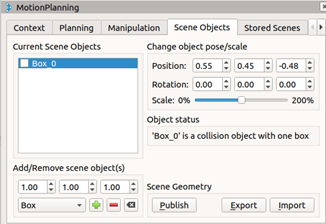
\includegraphics[width=10cm]{images/motionPlanning.png}
    \caption{Kinova RViz}\label{fig:kinovarviz}
    \end{figure}

Finally, publish the changes made so the move\_group instance saves the changes to include in planning stages.\\

\textbf{Deliverables:}

Use the interactive markers to move the gripper towards the planned scene object.

    \begin{enumerate}

        \item Describe what you see in terms of the pieces of robot changing colors.
        
        \textbf{Answer: }When the goal state has a potential collision with the scene object, the parts of the robot impacted will turn red. Mostly, the robot is divided by joints, so the changing color will apply to all the parts between two joints.  

        \item Hit the plan button (not execute) and report on any changes in the terminal or the status in the Planning tab.
        
        \textbf{Answer: } Upon hitting the button, the status in the Planning tab changes to 'Planning.' After 10 (or any times of your choosing) failed attempts, the status becomes 'Failed.' Generally, the planning is rather quick, but can be as thorough as possible.
    
    \end{enumerate}


\section{Pick and Place task}

Now that we have familiarized ourselves with the Kinova arm both in simulation and in the real world, we will expand our knowledge towards a common robotic arm task: pick and place.\\

\textbf{Instructions:}
For this portion of the assignment, we will return to the simulated Kinova Arm.

    \begin{minted}{bash}
       ~$ roslaunch kortex_gazebo spawn_kortex_robot.launch arm:=gen3_lite
    \end{minted}

In Gazebo, on the left panel’s “Insert” tab, find the “Wooden cube 7.5cm” object and add it to the world on a position on the ground within the robot arm’s workspace (space that can be reached by the arm).
Add another planned scene object, to avoid hitting the ground with the robot’s end effector. You can follow the same instructions from RViZ.
The pick and place task can be summarized in the following steps:
\begin{enumerate}
    \item Reach position above the center of the object to be picked with gripper oriented
    \item Adjust gripper to open or semi-open state.
    \item Decrease the end-effector’s z-value position
    \item Close gripper to grasp object.
    \item Reach position above the desired location to place the object with gripper oriented.
    \item Decrease the end-effector’s z-value position
    \item Open gripper to release object.
    \item Increase the end-effector’s z-value position to clear the object
    \item Return to home position.
    
\end{enumerate}

The goal of this section is to get familiar with this pick and place sequence and complete it step by step. To avoid errors during the executions, you are suggested to configure the program by running
\begin{minted}{bash}
       $ rosrun rqt_reconfigure rqt_reconfigure
    \end{minted}
Set allowed\_execution\_duration\_scaling to be 4 and uncheck the execution\_duration\_monitoring.
\begin{figure}[H]
    \vspace{-10pt}
    \centering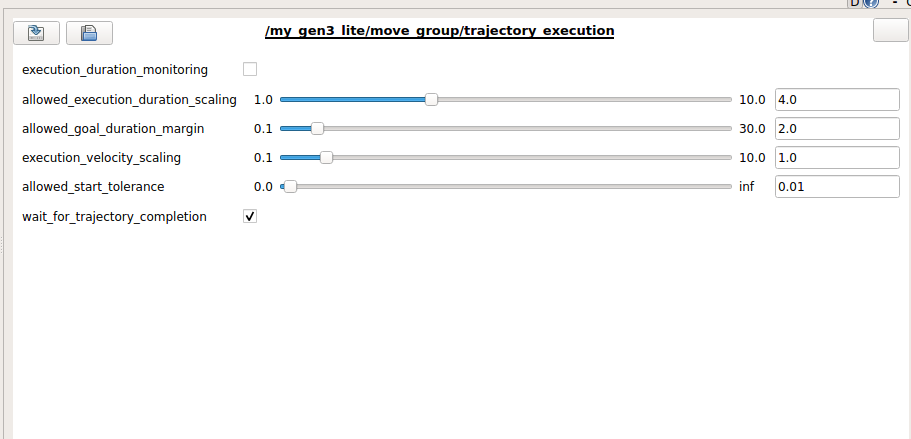
\includegraphics[width=13cm]{images/config.png}\vspace{-10pt}
    \caption{Configuration}\label{fig:kinovarviz}
    \end{figure}


\textbf{Deliverables:}

\begin{enumerate}

    \item Attempt the pick and place steps through RViZ. Report values of interest used to complete the task:
    
    \begin{enumerate}

        \item Pose of the cube and desired placing location.
        
        \textbf{Answer: }The initial position of the cube is somewhere around $(0.25, 0.25, 0)$, and the end position is just a quadrant away, around $(0.25, -0.25, 0)$.

        \item Selected height to approach object.
        
        \textbf{Answer: }The starting height of the arm is $0.25m$, and the lowered height to approach the object is around $0.06m$. Given the measurement of the cube is $7.5cm$, gripping height lower than $0.07m$ is likely safe.
        
        \item Percentage of the gripper’s open/close position.
        
        \textbf{Answer: }The open position of the gripper is $55\%$, default in the RViz setting. The close position for gripping, after trials and errors, is ideally $34\%$.

    \end{enumerate}

    \item Record a video of the completed task.
    
    \href{https://drive.google.com/file/d/1fpz9qItjWTIsZXeMqtLjGcoJgKeZQ377/view?usp=share_link}{Google Drive link to the simulated task of picking and placing the cube}

    \item Discuss some of the challenges you faced to complete the task.
    
    \textbf{Answer: }
    \begin{enumerate}
        \item One of the biggest challenges I face is the separation of interfaces. RViz is the place to plan for the motion of the arm and gripper, while Gazebo is the place to preview movement of all the models. It's been hard to tell whether the arm is at the right place to pick up the object of interest.
        \item Another challenge is the poor usability of RViz to navigate the arm. Directly setting the position parameters isn't allowed in the interface, and the only way is to use the interactive marker, which harms the accuracy of movement. Other actions, e.g. gripper percentages are also found out thru experiments.
        \item Finding the right spot to grasp the object is no easy task. Misalignment of the gripper and object positions leads to unexpected collisions; inappropriate gripper percentage can possibly destroy the object by squeezing or dropping it; Holding the object with the back of the grippers is slippery and risky, etc.
    \end{enumerate}

\end{enumerate}

\end{document}